% Created 2019-09-20 Пт 15:13
% Intended LaTeX compiler: pdflatex
\documentclass[11pt]{article}
\newcommand{\innp}[1]{\langle #1\rangle}
\usepackage{multirow}
\usepackage[utf8]{inputenc}
\usepackage[T1]{fontenc}
\usepackage{graphicx}
\usepackage{grffile}
\usepackage{longtable}
\usepackage{caption}
\usepackage{wrapfig}
\usepackage{rotating}
\usepackage[normalem]{ulem}
\usepackage{hyperref}
\usepackage{amsmath}
\usepackage{textcomp}
\usepackage{amssymb}
\usepackage{capt-of}
\usepackage{graphicx}
\usepackage{hyperref}
\usepackage[T2A]{fontenc}
\usepackage[a4paper,left=3cm,top=2cm,right=1.5cm,bottom=2cm,marginparsep=7pt,marginparwidth=.6in]{geometry}
\usepackage{cmap}
\usepackage[russian]{babel}
\usepackage{xcolor}
\usepackage{listings}
\usepackage{makecell}
\author{АВТОР}
\date{\today}
\title{}
\hypersetup{
 pdfauthor={АВТОР},
 pdftitle={},
 pdfkeywords={},
 pdfsubject={},
 pdfcreator={Emacs 26.1 (Org mode 9.1.9)}, 
 pdflang={Russian}}
\setcounter{page}{2}
{\renewcommand{\arraystretch}{1.5}
\begin{document}
\tableofcontents
\pagebreak
\section{Цель работы}
\begin{enumerate}
	\item Экспериментальная проверка равноускоренности движения тележки по наклонной плоскости.
	\item Определение величины ускорения свободного падения $g$.
\end{enumerate}
\section{Введение}
Как известно, при поступательном равноускоренном движении
тела вдоль оси $O$ зависимость проекции его скорости $v_x$ от времени $t$ определяется выражением:
$$v_x(t) = v_{0x} + a_xt \eqno(1)$$
где $v_{0x} $- проекция скорости на ось $O$ в момент времени $t = 0$,
$a_x$ -- ускорение тела. Зависимость координаты тела $x$ от времени
$t$ имеет вид:
$$\label{eq2} x(t) = x_0 + v_{0x}t + \frac{a_xt^2}{2} \eqno(2)$$
Здесь $x_0$ -- начальная координата. Если начальная скорость тела
равна нулю, то из (\ref{eq2}) следует:
$$ x_2 - x_1 = \frac{a}{2}(t_2^2-t_1^2) \eqno(3)$$
Таким образом, существует линейная зависимость между пе-
ремещением $\Delta x = x_2 - x_1$ и полуразностью квадратов значений
времени $\frac{t_2^2-t_1^2}{2}$ Коэффициент пропорциональности этой зависимости равен ускорению тела. Если экспериментальный график этой
зависимости будет представлять собой прямую линию, то это будет доказательством движения с постоянным ускорением.
В качестве объекта совершающего равнопеременное поступательное движение рассмотрим тележку, скользящую по наклонной
плоскости (см. рис.(\hyperref[im1]{1}). Второй закон Ньютона, описывающий ее
движение, имеет вид:
$$\label{eq4} m\vec{a}=m\vec{g}+\vec{N}+\vec{F_{тр}} \eqno(4)$$
где $\vec{a}$ -- ускорение тележки, $\vec{N}$ -- сила реакции опоры, а сила трения, возникающая при скольжения, по модулю равна произведению
коэффициента трения на силу нормальной реакции: $F_{тр} = \mu N$. Проекции уравнения (\hyperref[eq4]{4})  на координатные оси:
\begin{equation*}
	\label{eq5}
	\begin{cases}
		O_y : N - mg \cos \alpha\\
		O_x : ma = mg \sin \alpha - \mu mg \cos \alpha
	\end{cases}
	\eqno(5)
\end{equation*}
где $\alpha$ -- угол между наклонной плоскостью и горизонталью. Из
(\hyperref[eq5]{5}) следует выражение для модуля ускорения:
$$\label{eq6} a = g \sin \alpha - \mu \cos \alpha \eqno(6)$$
\begin{figure}[hp]
	\centering
	\captionsetup{justification=centering}
	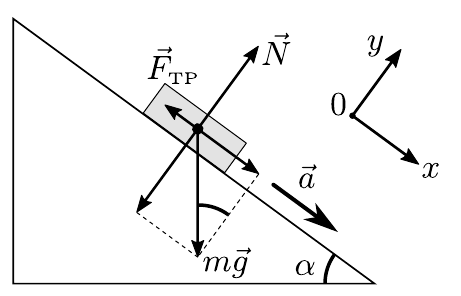
\includegraphics[width=120px]{im1.png}
	\caption{Векторная диаграмма сил, действующих на тело,расположенное на наклонной плоскости}
	\label{im1}
\end{figure}
\pagebreak
Поскольку в лабораторной установке коэффициент трения $\mu$и
угол $\alpha$ достаточно малы, то $cos \alpha$ в формуле(\hyperref[eq6]{6}) можно заменить
единицей. С учетом этого выражение для ускорения будет иметь вид:
$$ a = g(\sin \alpha - \mu) \eqno(7)$$
Таким образом, теоретическая зависимость ускорения $a$ от
$\sin \alpha$ является линейной и угловой коэффициент этой зависимо-
сти равен ускорению свободного падения $g$.
\section{Измерительные приборы}
\begin{table}[htb]
\centering
\large
\caption{Измерительные приборы}
	\begin{tabular}{|c|c|c|c|c|}
		\hline
		\textbf{Наименование} & \makecell{\textbf{Предел}\\ \textbf{измерений}} & \makecell{\textbf{Цена}\\ \textbf{деления}} & \makecell{\textbf{Класс}\\ \textbf{точности}} & $\Delta$\textsubscript{и}\\
		\hline
		Линейка на рельсе  & $1,3$ \textit{м} & $1$ \textit{cм}/\textit{дел} & --- & $5$ \textit{мм}\\
		\hline
		Линейка на угольнике  & $250$ \textit{мм} & $1$ \textit{мм}/\textit{дел} & --- & $0,5$ \textit{мм}\\
		\hline
		ПКЦ-3 в режиме секундомера   & $100$ \textit{c} & $0,1$ \textit{c} & --- & $0,1$ \textit{c}\\
		\hline
	\end{tabular}
\end{table}
\section{Результаты прямых измерений}
Настоящий протокол с измерений с подписью приводится как Приложение 1 (один лист, заполненный от руки с двух сторон).
\begin{table}[htb]
\centering
\large
\caption{}
\begin{tabular}{|c|c|c|c|}
		\hline
		$x,$ \textit{м} & $x',$ \textit{м} & $h_0,$ \textit{мм}  & $h'_0,$ \textit{мм}\\
		\hline
		$0,22 \pm 0,005$& $1,0 \pm 0,005$& $196\pm 0,5$ &$ 194 \pm 0,5$\\
		\hline
	\end{tabular}
\end{table}
\begin{table}[htb]
	\caption{Результаты прямых измерений (Задание 1)}
	\centering
	\large
	\begin{tabular}{|c|c|c|c|c|c|c|}
		\hline
		\multirow{2}{*}{\textnumero} & \multicolumn{4}{c}{Измеренные величины} & \multicolumn{2}{|c|}{Рассчитанные величины}\\
		\cline{2-7}
						      & $x_1,$ \textit{м}  & $x_2,$ \textit{м}  & $t_1, c$  & $t_2, c$   & $x_2 - x_1, $ \textit{м} & $\frac{t^2_{2} - t^2_1}{2}, c^2$\\
		\hline
		1 & $0,15 \pm 0,005$ & $0,40 \pm 0,005$ & $1,3 \pm 0,1$ & $2,6 \pm 0,1$ & $0,25 \pm 0,005$ & $2,54  \pm 0,005$\\
		\hline
		2 & $0,15 \pm 0,005$ & $0,50 \pm 0,005$ & $1,2 \pm 0,1$ & $2,9 \pm 0,1$ & $0,35 \pm 0,005$ & $3,49  \pm 0,005$\\
		\hline
		3 &$0,15 \pm 0,005$ & $0,70 \pm 0,005$ & $1,3 \pm 0,1$& $3,6 \pm 0,1$ & $0,55 \pm 0,005$ & $5,64  \pm 0,005$\\
		\hline
		4 & $0,15 \pm 0,005$ & $0,90 \pm 0,005$ & $1,3 \pm 0,1$& $4,1 \pm 0,1$ & $0,75 \pm 0,005$ & $7,56  \pm0,005$\\
		\hline
		5 & $0,15 \pm 0,005$ & $1,10 \pm 0,005$ & $1,2 \pm 0,1$& $4,6 \pm 0,1$ &$0,95 \pm 0,005$  & $9,86  \pm 0,005$\\
		\hline
	\end{tabular}
\end{table}

{\renewcommand{\arraystretch}{1.3}
\pagebreak
\begin{table}[htb]
	\caption{Результаты прямых измерений (Задание 2)}
	\centering
	\large
	\begin{tabular}{|c|c|c|c|c|c|}
		\hline
		N\textsubscript{ПЛ} & $h$,  \textit{мм}& $h'$,  \textit{мм}& \textnumero & $t_1, c$ & $t_2, c$\\
		\hline
		\multirow{5}{*}{1} & \multirow{5}{*}{187} & \multirow{5}{*}{193} & 1 & $1,2$ & $4,5$\\	
		\cline{4-6}
		&&& 2 & $1,3$ & $4,6$\\
		\cline{4-6}
		&&& 3 & $1,2$ & $4,5$\\
		\cline{4-6}
		&&& 4 & $1,3$ & $4,6$\\
		\cline{4-6}
		&&& 5 & $1,4$ & $4,7$\\
		\hline
		\multirow{5}{*}{2} & \multirow{5}{*}{178} & \multirow{5}{*}{193} & 1 & $0,9$ & $3,2$\\	
		\cline{4-6}
		&&& 2 & $0,9$ & $3,2$\\
		\cline{4-6}
		&&& 3 & $0,8$ & $3,1$\\
		\cline{4-6}
		&&& 4 & $0,9$ & $3,2$\\
		\cline{4-6}
		&&& 5 & $0,9$ & $3,2$\\
		\hline
		\multirow{5}{*}{3} & \multirow{5}{*}{169} & \multirow{5}{*}{193} & 1 & $0,7$ & $2,6$\\	
		\cline{4-6}
		&&& 2 & $0,7$ & $2,6$\\
		\cline{4-6}
		&&& 3 & $0,7$ & $2,5$\\
		\cline{4-6}
		&&& 4 & $0,7$ & $2,5$\\
		\cline{4-6}
		&&& 5 & $0,7$ & $2,5$\\
		\hline
		\multirow{5}{*}{4} & \multirow{5}{*}{160} & \multirow{5}{*}{192} & 1 & $0,7$ & $2,2$\\	
		\cline{4-6}
		&&& 2 & $0,6$ & $2,1$\\
		\cline{4-6}
		&&& 3 & $0,7$ & $2,1$\\
		\cline{4-6}
		&&& 4 & $0,7$ & $2,2$\\
		\cline{4-6}
		&&& 5 & $0,7$ & $2,2$\\
		\hline
		\multirow{5}{*}{5} & \multirow{5}{*}{151} & \multirow{5}{*}{192} & 1 & $0,7$ & $2,0$\\	
		\cline{4-6}
		&&& 2 & $0,7$ & $2,0$\\
		\cline{4-6}
		&&& 3 & $0,7$ & $2,0$\\
		\cline{4-6}
		&&& 4 & $0,7$ & $2,0$\\
		\cline{4-6}
		&&& 5 & $0,7$ & $2,0$\\
		\hline
	\end{tabular}
\end{table}
\section{Обработка результатов измерений}
\subsection{Задание 1}
\begin{enumerate}
	\item Величины $Y = x_2 - x_1$ и $Z = \frac{t^2_2 - t^2_1}{2}$ и их погрешности записаны в Табл. 3 .
	\item График теоритической зависимости $Y = aZ$ c угловым коэффициентом равным ускорению приведён в Приложении 2 как График 1.
	\item Вычислим коэффициент $a$ его среднеквадратическое отклонение (СКО) $\sigma_{\innp{a}}$ :
		$$\frac{\sum\limits_{i=1}^N Z_iY_i}{\sum\limits_{i=1}^N Z_i^2};  \quad \sigma_{\innp{a}} = \sqrt{\frac{\sum\limits_{i=1}^N(Y_i-aZ_i)^2}{(N-1)\sum\limits_{i=1}^N Z^2_i}} \eqno(8)$$
		где $N$– количество экспериментальных точек, в данной серии измерений $N$= 5.
		Угловой коэффициент $a = 0,1$ и $\sigma_{\innp{a}} =  2,73 \cdot 10^{-3}$\\
		Абсолютную погрешность коэффициента $a$ для доверительной вероятности $\alpha = 0,95$ вычислим по формуле:
		$$\Delta_a = t_{\alpha,N-1} \cdot \sigma_{a}, \eqno(9)$$
		где - $ t_{\alpha,N-1}$ коэффициент Стьюдента для доверительной вероятности $\alpha$ и количества измерений 	N.
		$ t_{\alpha,N-1} = 2,78$ соотствественно $\Delta_a = 7,59 \cdot 10^{-3}$.
		Вычислим относительную погрешность ускорения по формуле:	
		$$\varepsilon_a = \frac{\Delta_a}{a} \cdot 100\% \eqno(10)$$
		$\varepsilon_a = 7,59$
	\item Зависимость $Y(Z) = aZ$ построена на Графике 1.
\end{enumerate}
\subsubsection{Вывод}
Так как зависимость $Y(Z) = aZ$ линейна, то движение тележки равноускоренное.
\subsection{Задание 2}
\begin{enumerate}
	\item  Для каждой серии измерений из Таблицы 4 вычислим значение  синуса угла наклона рельса к горизонту по формуле:
$$\sin \alpha = \frac{(h_0-h)-(h'_0-h')}{x' - x} \eqno(11)$$
	\item Вычислим средние значения времени $t_1$ и $t_2$ каждой серии и их погрешности по формулам:
			$$\innp{t} = \frac{1}{N}\sum\limits_{i=1}^Nt_{i} \eqno(12)$$
			СКО:
				$$\sigma_{\innp{t}} = \sqrt{\frac{\sum\limits_{i=1}^N(t_i - \innp{t})^2}{N(N-1)}} \eqno(13)$$
			Cлучайная погрешность:
				$$\Delta_{\innp{t}} = t_{\alpha,N} \cdot \sigma_{\innp{t}} \eqno(14)$$
			Абсолютная погрешность:
				$$\Delta_t = \sqrt{\Delta_{\innp{t}}^2 + \Big(\frac{2}{3} \cdot \Delta_{\text{и}}\Big)^2} \eqno(15)$$
	\item Вычислим значение ускорения и его погрешность для каждой
		серии измерений по формулам:
				$$ \innp{a} = \frac{2(x_2-x_1)}{{\innp{t_2}}^2 -{\innp{t_1}}^2 }\eqno(16)$$
				$$\Delta_a = \innp{a} \cdot \sqrt{\frac{{(\Delta_{x\text{и}2})}^2 + {(\Delta_{x\text{и}1})}^2}{(x_2-x_1)^2} + 4 \cdot \frac{{(\innp{t_1} \Delta_{t_1})}^2 + {(\innp{t_2} \Delta_{t_2})}^2}{({\innp{t_2}}^2 - {\innp{t_1}}^2)^2}} \eqno(17)$$
		где $\Delta_{x\text{и}1}$ и $\Delta_{x\text{и}2}$ – приборные погрешности измерения координат
		 и $x_1$ и $x_2$; $\Delta_{t_1}$ и $\Delta_{t_2}$-- абсолютные погрешности значений времен
		$t_1$ и $t_2$.
	\item Результаты расчетов для ускорения внесены в таблицу.
	\end{enumerate}
	\pagebreak
		\begin{table}[htb]
			\centering
			\caption{Результаты расчетов (Задание 2)}
			\begin{tabular}{|c|c|c|c|c|}
				\hline
				N\textsubscript{ПЛ} & $\sin \alpha$& $\innp{t_1} \pm \Delta t_1$, \textit{c} & $\innp{t_2} \pm \Delta t_2$, \textit{c} & $\innp{a} \pm \Delta a$, $\frac{\textup{м}}{\textup{c}^2}$\\
				\hline
				1 & 0,010& $1,3 \pm 0,130$& $4,6 \pm 0,130$& $0.098 \pm 0.028$\\
				\hline
				2 & 0,022& $0,9 \pm 0,087$& $3,2 \pm 0,087$& $0.201\pm 0,038$\\
				\hline
				3 & 0,033& $0,7 \pm 0,067$& $2,5 \pm 0,107$& $0.330\pm 0,075$\\
				\hline
				4 & 0,044& $0,7 \pm 0,087$& $2,2 \pm 0,107$& $0.437\pm 0,102$\\
				\hline
				5 & 0,055& $0,7 \pm 0,067$& $2,0 \pm 0,067$& $0.541\pm 0,082$\\
				\hline
			\end{tabular}
		\end{table}
\begin{enumerate}
	\setcounter{enumi}{4}
	\item Теоритическая зависимость $a$ от $\sin \alpha$ имеет линейный характер: $a = A + B \sin \alpha$, где $A = -\mu g$, $B = g$ (следует из (7)).
	Вычислим $g$ методом наименьших квадратов (МНК).
	Найдем среднее значение синуса и ускорения:
		$$\innp{\sin \alpha} = \frac{1}{N} \sum\limits_{i=1}^N\sin \alpha_i; \quad \innp{a} = \frac{1}{N} \sum\limits_{i=1}^N a_i \eqno(18)$$
	$\innp{\sin \alpha} = 0,033; \quad \innp{a} = 0,321$
	Найдём коэффициенты линейной зависимости по следующим
	формулам:
	$$ B = \frac{\sum\limits_{i=1}^N (\sin{\alpha_i} - \innp{\sin{\alpha}})(a_i - \innp{a})}{\sum\limits_{i=1}^N {(\sin{\alpha_i} - \innp{\sin{\alpha_i}})}^2}; \quad A = \innp{a} - B\innp{\sin \alpha} \eqno(19)$$
$B = 10,012 \quad A = -0,009$\\
Рассчитаем параметры $d_i$ и $D$ по формулам:
$$ d_i = a_i - (A + B \sin{\alpha_i}), \eqno(19)$$
$$ D = \sum\limits_{i=1}^N {(\sin{\alpha_i} - \innp{\sin{\alpha_i}})}^2  \eqno(20)$$
Вычислим СКО коэффициента $B$:
	$$ \sigma_B = \sqrt{\frac{\sum\limits_{i=1}^N d_i^2}{D(N-2)}} \eqno(21)$$
$\sigma_B = 0.261$
Определим абсолютную погрешность коэффициента $B$ для доверительной вероятности $\alpha = 0,95$ по формуле:
	$$\Delta B = t_{\alpha, N-2} \cdot \sigma_B \eqno(22)$$
$\Delta B = 1.122$\\
Рассчитаем относительную погрешность коэффициента $B$:
	$$\varepsilon_B = \frac{\Delta B}{B} \cdot 100\% \eqno(23)$$
	$\varepsilon_B = 11,207$
\end{enumerate}
\pagebreak
\begin{enumerate}
	\setcounter{enumi}{5}
	\item Найдем абсолютную и относительную погрешность полеченного g от его
табличного значения по формулам:
		$$\Delta g = g_{\text{эксп}} - g_{\text{табл}}  \eqno(24)$$
		$$\varepsilon_g = \frac{\Delta g}{g_{\text{табл}}}  \eqno(25)$$
	$\Delta g = 0,205 \quad \varepsilon_g = 2,090$
	\item $\Delta g$ = $ | g_{\text{эксп}} - g_{\text{табл}}|$
\subsubsection{Вывод}
Получено g, близкое по значению к табличному с учётом погрешности
\end{enumerate}
Зависимости $a(\sin \alpha) = a$ и $a = A + B\sin \alpha$ приведены на Графике 2 в Приложении 2
\section{Результаты лабораторной работы}
\begin{enumerate}
\item Графики приведены в Приложении 2.
\item Доверительный интервала для ускорения, полученный в первом задании, с относительной погрешностью:
	$$\Delta_a = 7,59 \cdot 10^{-3}; \quad \varepsilon_a = 7,59$$
\item Значение ускорения свободного падения с абсолютной и относительной погрешностями:
	$$ g = 10,012; \quad \Delta g = 1,122; \quad \varepsilon_g = 11,207$$
\item Абсолютное и относительное отклонение измеренного ускорения свободного падения от его табличного значения:
$$\Delta g = 0,205 \quad \varepsilon_g = 2,090$$
\end{enumerate}
\end{document}